\section{Objective}
    The goal of this research project was to enable the determination of resonance parameters for the unresolved resonance region (URR) directly from self-shielded measurements. To accomplish this, this project involved the verification and validation of the self-shielding code SESH\cite{sesh}, which was then integrated into the nuclear resonance parameter fitting code SAMMY\cite{sammy}.


\section{Problem Description}

    In nuclear engineering, the cross section can essentially be broken up into three regions: the resolved resonance region, the unresolved resonance region, and the fast region. The resolved resonance region is where nuclear resonances can be resolved experimentally. The fast region is where we have a smooth cross section. The unresolved resonance region is where resonances cannot be resolved experimentally, but in which the resonant structure still is experimentally observed. The resonant structure in the URR is accounted for in neutron transport codes by the use of probability tables. These probability tables are essentially a histogram of different possible cross section values for any given energy. The histograms which make up these probability tables are populated by simulating cross section resonances in the URR based on average resonance parameters and the parameters' known statistical distributions. NJOY\cite{njoy} is one such code that is responsible for generating these histograms from average resonance parameters. Accounting for resonant structure is essential for correctly modeling critical systems.





    Consider the IMF-10 Criticality Benchmark\cite{icsbep}, which is a 9\% enriched cylindrical system with a depleted uranium reflector. This was modeled in MCNP using cross sections generated from the ENDF-VIII.0 nuclear data library\cite{endf-8} and processed with NJOY. In order to show the effect of the URR resonant structure, the benchmark was run once with the probability tables enabled and once with the probability tables disabled.

    \begin{table}[h!]
        \centering
        \caption{Impact of the URR on the ZPR-U9 Criticality Benchmark.}
        \begin{tabular}{|l  c  c|}
            \hline
            ~                       &   $k_{eff}$   & $\Delta \rho$ (pcm) \\
            \hline
            URR P-Tables Enabled    &   $1.00274$   & $0$ \\
            URR P-Tables Disabled   &   $0.99806$   &   $-467$ \\
            \hline
        \end{tabular}
        \label{tab:criticality-benchmark}
    \end{table}
    
    The results are given in \autoref{tab:criticality-benchmark}. In this example, the effect of accounting for URR fluctuations compared to not accounting for URR fluctuations reduced the reactivity of the system by 467 pcm. This difference in criticality is referred to as resonance self-shielding.

    While accounting for resonant fluctuations in the URR is straightforward once accurate average resonance parameters are determined, self-shielding is still going to be encountered when taking measurements in the URR. Essentially, due to the non-linearity of the cross section and the functional form of the measurements of said cross section, the average measured quantity is not equal to the measurement of the average cross section. Put more concretely, this non-equivalence can be stated as the average value of a transmission measurement is not equal to the transmission of the average cross section, or
    \begin{equation}
        \label{eq:self-shielding}
        \langle T (\sigma) \rangle \neq T(\langle \sigma \rangle)
    \end{equation}
    in which $\langle ... \rangle$ represents a quantity averaged over some energy region.
    
    This issue is shown in \autoref{fig:self-shielding-demo}, using \textsuperscript{181}Ta as an example. Here, the transmission of a 0.105 at/barn thick sample is simulated in three ways. First, in which the $\sigma(E)$ was finely resolved, such that a true $T(E)$ was obtained. Second, in which the transmission is obtained as an energy-averaged quantity, $\langle T \rangle$. Finally, the energy-average of the known cross section $\langle \sigma \rangle$ was obtained over the same energy region and the ``transmission of the average cross section'' was calculated, $e^{-n \langle \sigma \rangle}$. The two average quantities, $\langle T\rangle$ and $e^{-n \langle \sigma \rangle}$, not being equal is exactly what prevents the use of a nuclear fitting code like SAMMY\cite{sammy} to be used with URR measurements that have not accounted for self-shielding.

    \begin{figure}
        \centering
        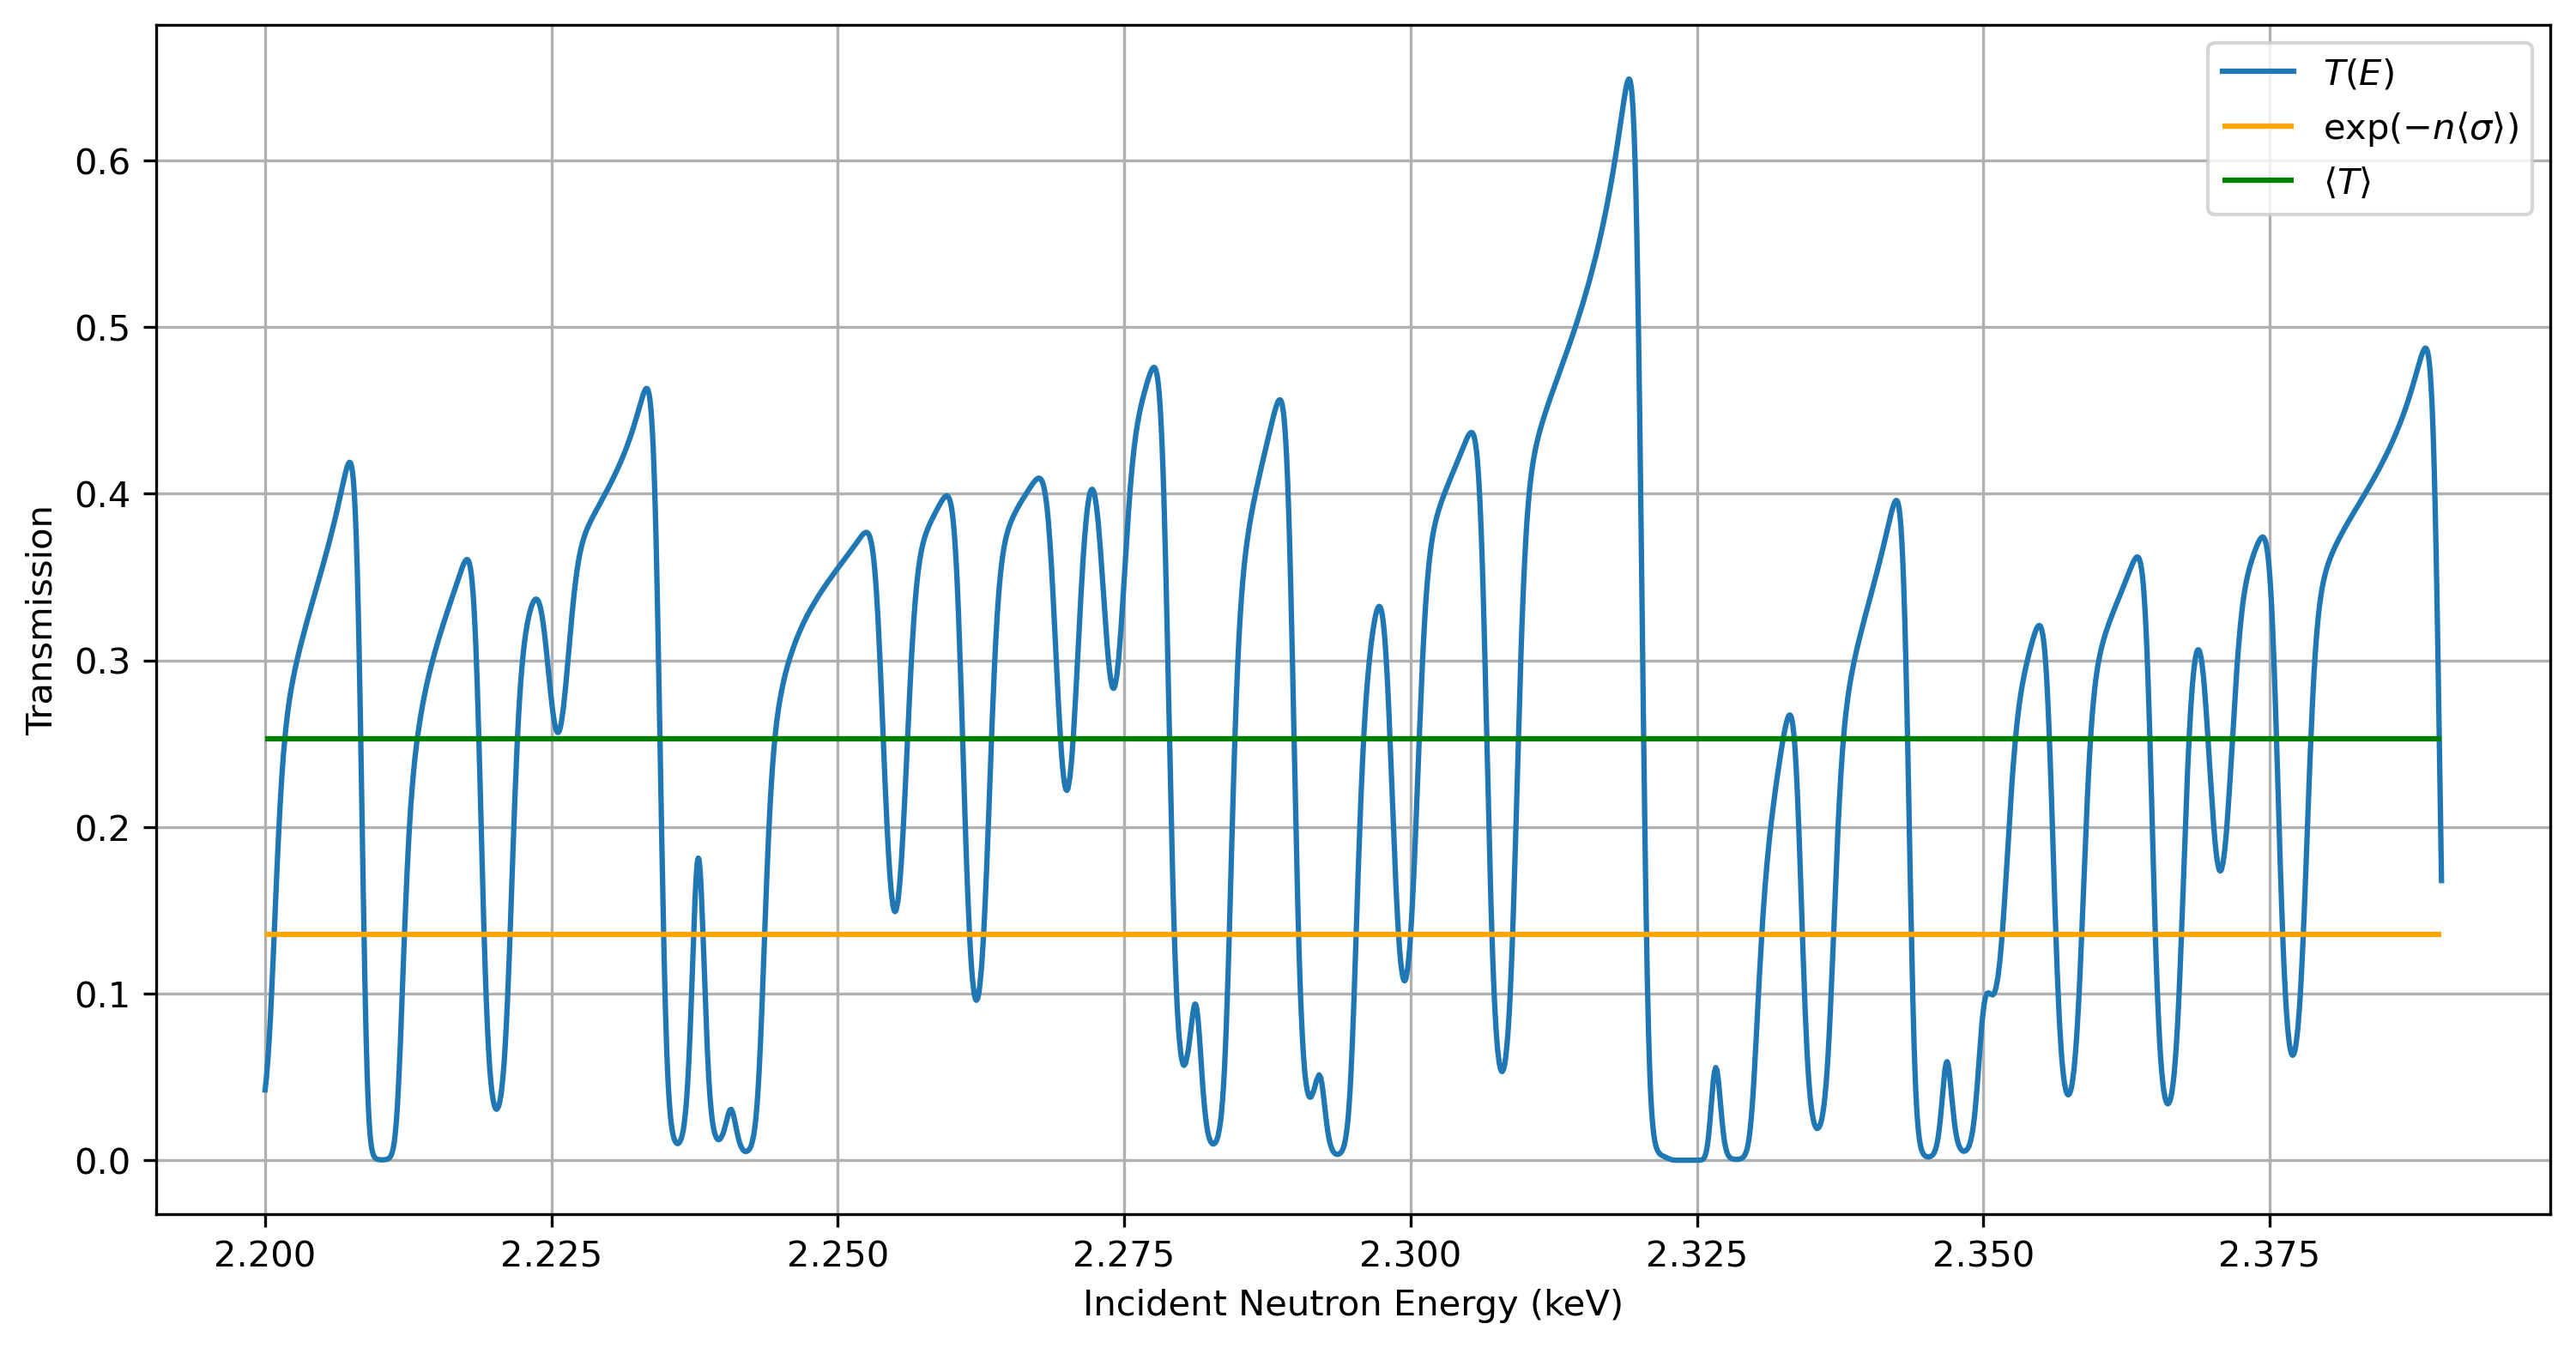
\includegraphics[width=0.95\textwidth]{Introduction/Figures/transmission-example.png}
        \caption{Demonstration of Self-Shielding for \textsuperscript{181}Ta comparing the `True Transmission' (blue line), `Average Transmission' (green line), and `Transmission of Average Cross Section' (orange line).}
        \label{fig:self-shielding-demo}
    \end{figure}

    To summarize, three facts are true:
    \begin{enumerate}
        \item The resonant structure in the URR cannot be ignored in modeling critical systems.
        \item Modeling the resonant structure in the URR requires accurate resonance parameters.
        \item URR parameters cannot be directly determined from transmission and capture experiments due to self-shielding.
    \end{enumerate}

    Therefore, a problem remains: how can an average measurement be expressed as a function of the average cross section? It wouldn't be sufficient to fit resonance parameters using the ``uncorrected'' cross-section, i.e.,
    \begin{equation}
        \overline{\sigma} = -\frac{1}{n} \ln{\langle T \rangle}
    \end{equation}
    as this value is heavily dependent on experimental conditions such as temperature and sample thickness, and does not account for self-shielding. The resonance parameters obtained from fitting $\overline{\sigma}$ would not accurately represent the true cross section.

    If resonance parameters which accurately describe the true average cross section are to be obtained, self-shielding must be accounted for. In order to do that, a correction factor is used, such that
    \begin{equation}
        \label{eq:self-shielded-transmission}
        \langle T \rangle = e^{-n \langle \sigma \rangle} C_T
    \end{equation}
    This `transmission correction factor', $C_T$, corrects for the self-shielding effect produced by the resonant fluctuations in the URR.

    This project integrated self-shielding correction factors directly into SAMMY, enabling the code to fit self-shielded URR transmission and capture yield measurements. Additionally, the capability to fit multiple isotope samples, such as self-shielded transmission and capture measurements of natural samples, was introduced: a feature not previously available in SAMMY's URR fitting. This new functionality significantly modernized SAMMY's URR fitting interface. This developed package was then applied to a new evaluation of the unresolved resonance region for Zr\textsuperscript{90} and Zr\textsuperscript{91}, utilizing natural datasets to improve the performance of the fit, which had been previously impossible due to the lack of multi-isotope functionality.